\title{Mixture density networks}

\subsection{Mixture density networks}

Mixture density networks (MDN) \citep{bishop1994mixture} are a class
of models obtained by combining a conventional neural network with a
mixture density model.

We demonstrate how to use MDNs in Edward, leveraging TensorFlow Slim
to construct neural networks.
The script is available
\href{https://github.com/blei-lab/edward/blob/master/examples/mixture_density_network.py}
{here}.

\subsubsection{Data}

We use the same toy data from the
\href{http://blog.otoro.net/2015/11/24/mixture-density-networks-with-tensorflow/}{David
Ha's blog post}, where he explains MDNs. It is an inverse problem where
for every input $x_n$ there are multiple outputs $y_n$.

\begin{lstlisting}[language=Python]
def build_toy_dataset(N):
  y_data = np.random.uniform(-10.5, 10.5, N).astype(np.float32)
  r_data = np.random.normal(size=N).astype(np.float32)  # random noise
  x_data = np.sin(0.75 * y_data) * 7.0 + y_data * 0.5 + r_data * 1.0
  x_data = x_data.reshape((N, 1))
  return train_test_split(x_data, y_data, random_state=42)

N = 5000  # number of data points
D = 1  # number of features

X_train, X_test, y_train, y_test = build_toy_dataset(N)
print("Size of features in training data: {}".format(X_train.shape))
print("Size of output in training data: {}".format(y_train.shape))
print("Size of features in test data: {}".format(X_test.shape))
print("Size of output in test data: {}".format(y_test.shape))

sns.regplot(X_train, y_train, fit_reg=False)
\end{lstlisting}

\begin{lstlisting}
## Size of features in training data: (3750, 1)
## Size of output in training data: (3750,)
## Size of features in test data: (1250, 1)
## Size of output in test data: (1250,)
\end{lstlisting}

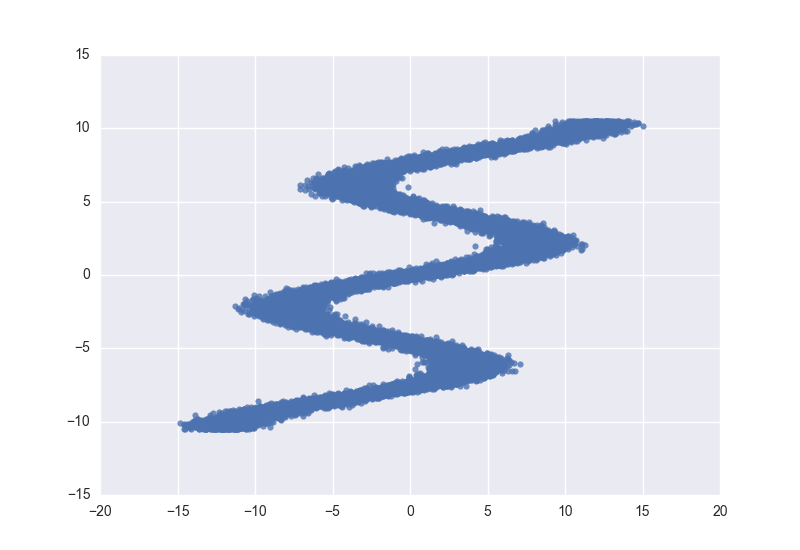
\includegraphics[width=650px]{/images/mdn-fig0.png}

We define TensorFlow placeholders, which will be used to manually feed batches of data during inference. This is \href{http://edwardlib.org/api/data}{one of many ways} to train models with data in Edward.

\begin{lstlisting}[language=Python]
X_ph = tf.placeholder(tf.float32, [None, D])
y_ph = tf.placeholder(tf.float32, [None])
\end{lstlisting}

\subsubsection{Model}

We use a mixture of 20 normal distributions parameterized by a
feedforward network. That is, the membership probabilities and
per-component mean and standard deviation are given by the output of a
feedforward network.  We specify a three-layer network with 15 hidden
units for each hidden layer.

\begin{lstlisting}[language=Python]
def neural_network(X):
  """mu, sigma, logits = NN(x; theta)"""
  # 2 hidden layers with 15 hidden units
  hidden1 = slim.fully_connected(X, 15)
  hidden2 = slim.fully_connected(hidden1, 15)
  mus = slim.fully_connected(hidden2, K, activation_fn=None)
  sigmas = slim.fully_connected(hidden2, K, activation_fn=tf.exp)
  logits = slim.fully_connected(hidden2, K, activation_fn=None)
  return mus, sigmas, logits

K = 20  # number of mixture components

mus, sigmas, logits = neural_network(X_ph)
cat = Categorical(logits=logits)
components = [Normal(mu=mu, sigma=sigma) for mu, sigma
              in zip(tf.unstack(tf.transpose(mus)),
                     tf.unstack(tf.transpose(sigmas)))]
y = Mixture(cat=cat, components=components, value=tf.zeros_like(y_ph))
\end{lstlisting}

Note that we use the \texttt{Mixture} random variable. It collapses
out the membership assignments for each data point and makes the model
differentiable with respect to all its parameters. It takes a
\texttt{Categorical} random variable as input—denoting the probability for each
cluster assignment—as well as \texttt{components}, which is a list of
individual distributions to mix over.

For more background on MDNs, take a look at
\href{http://cbonnett.github.io/MDN.html}{Christopher Bonnett's blog
post} or at \citet{bishop1994mixture}.

\subsubsection{Inference}

We use MAP estimation, passing in the model and data set.
See this extended tutorial about
\href{/tutorials/map}{MAP estimation in Edward}.

\begin{lstlisting}[language=Python]
inference = ed.MAP(data={y: y_ph})
\end{lstlisting}

Here, we will manually control the inference and how data is passed
into it at each step.
Initialize the algorithm and the TensorFlow variables.

\begin{lstlisting}[language=Python]
inference.initialize(var_list=tf.trainable_variables())

sess = ed.get_session()
tf.global_variables_initializer().run()
\end{lstlisting}

Now we train the MDN by calling \texttt{inference.update()}, passing
in the data. The quantity \texttt{inference.loss} is the
loss function (negative log-likelihood) at that step of inference. We
also report the loss function on test data by calling
\texttt{inference.loss} and where we feed test data to the TensorFlow
placeholders instead of training data.
We keep track of the losses under \texttt{train\_loss} and \texttt{test\_loss}.

\begin{lstlisting}[language=Python]
n_epoch = 1000
train_loss = np.zeros(n_epoch)
test_loss = np.zeros(n_epoch)
for i in range(n_epoch):
  info_dict = inference.update(feed_dict={X_ph: X_train, y_ph: y_train})
  train_loss[i] = info_dict['loss']
  test_loss[i] = sess.run(inference.loss, feed_dict={X_ph: X_test, y_ph: y_test})
  inference.print_progress(info_dict)
\end{lstlisting}

After training for a number of iterations, we get out the predictions
we are interested in from the model: the predicted mixture weights,
cluster means, and cluster standard deviations.

To do this, we fetch their values from session, feeding test data
\texttt{X_test} to the placeholder \texttt{X_ph}.

\begin{lstlisting}[language=Python]
pred_weights, pred_means, pred_std = \
    sess.run([tf.nn.softmax(logits), mus, sigmas], feed_dict={X_ph: X_test})
\end{lstlisting}

Let's plot the log-likelihood of the training and test data as
functions of the training epoch. The quantity \texttt{inference.loss}
is the total log-likelihood, not the loss per data point.  In the
plotting routine we get the latter by dividing by the size of the
train and test data respectively.

\begin{lstlisting}[language=Python]
fig, axes = plt.subplots(nrows=1, ncols=1, figsize=(16, 3.5))
plt.plot(np.arange(n_epoch), -test_loss / len(X_test), label='Test')
plt.plot(np.arange(n_epoch), -train_loss / len(X_train), label='Train')
plt.legend(fontsize=20)
plt.xlabel('Epoch', fontsize=15)
plt.ylabel('Log-likelihood', fontsize=15)
plt.show()
\end{lstlisting}

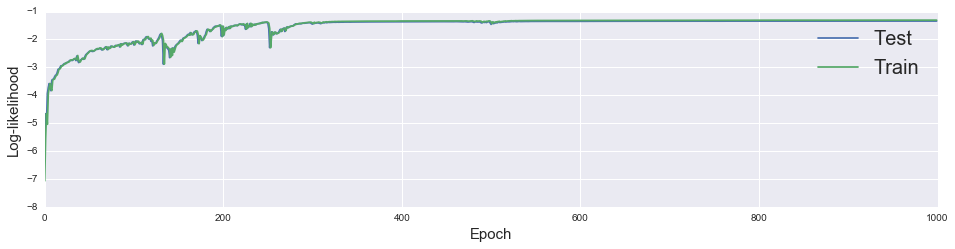
\includegraphics[width=700px]{/images/mdn-fig1.png}

We see that it converges after 400 iterations.

\subsubsection{Criticism}

Let's look at how a few individual examples perform. Note that as this
is an inverse problem we can't get the answer correct, but we can hope
that the truth lies in area where the model has high probability. This code relies on helper functions
available in the full script above.

In this plot the truth is the vertical grey line while the blue line is the prediction of the mixture density network. As you can see, we didn't do too bad.

\begin{lstlisting}[language=Python]
obj = [0, 4, 6]
fig, axes = plt.subplots(nrows=3, ncols=1, figsize=(16, 6))

plot_normal_mix(pred_weights[obj][0], pred_means[obj][0], pred_std[obj][0], axes[0], comp=False)
axes[0].axvline(x=y_test[obj][0], color='black', alpha=0.5)

plot_normal_mix(pred_weights[obj][2], pred_means[obj][2], pred_std[obj][2], axes[1], comp=False)
axes[1].axvline(x=y_test[obj][2], color='black', alpha=0.5)

plot_normal_mix(pred_weights[obj][1], pred_means[obj][1], pred_std[obj][1], axes[2], comp=False)
axes[2].axvline(x=y_test[obj][1], color='black', alpha=0.5)
\end{lstlisting}

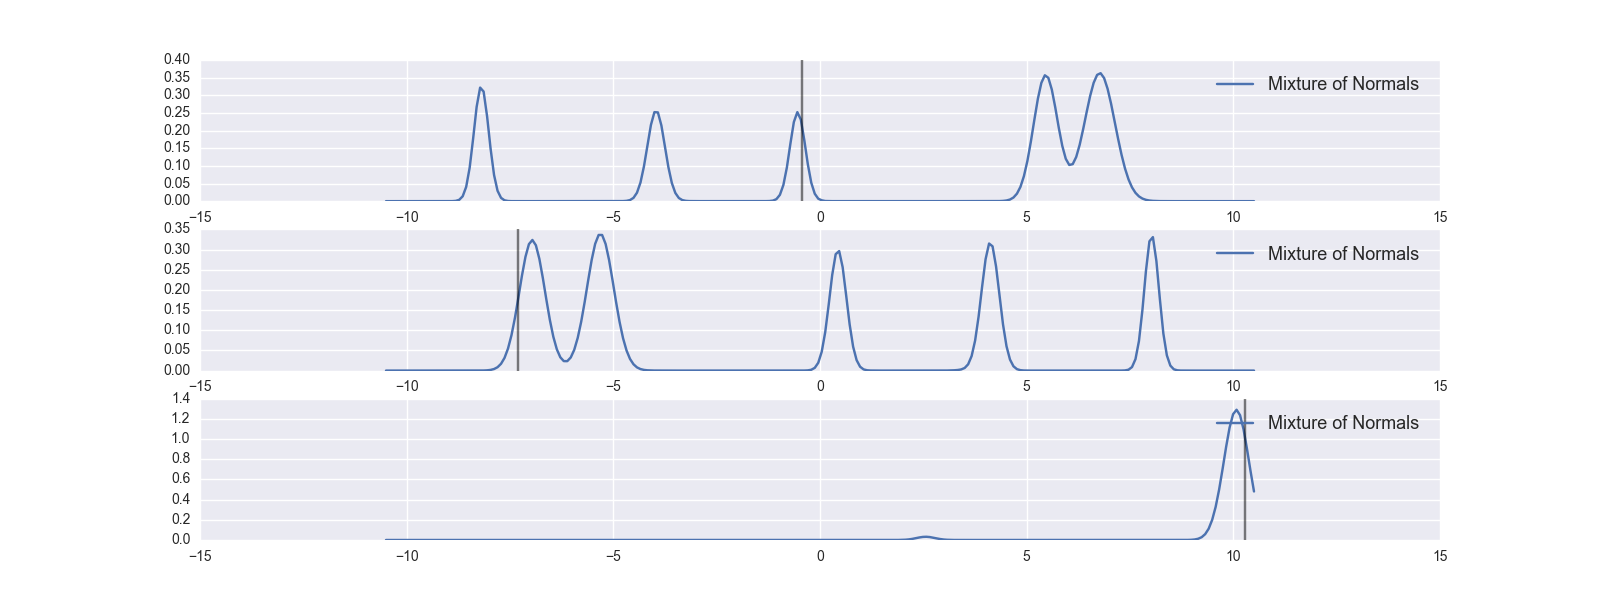
\includegraphics[width=700px]{/images/mdn-fig2.png}

We can check the ensemble by drawing samples of the prediction and
plotting the density of those. The MDN has learned what we'd like it
to learn.

\begin{lstlisting}[language=Python]
a = sample_from_mixture(X_test, pred_weights, pred_means, pred_std, amount=len(X_test))
sns.jointplot(a[:,0], a[:,1], kind="hex", color="#4CB391", ylim=(-10,10), xlim=(-14,14))
\end{lstlisting}

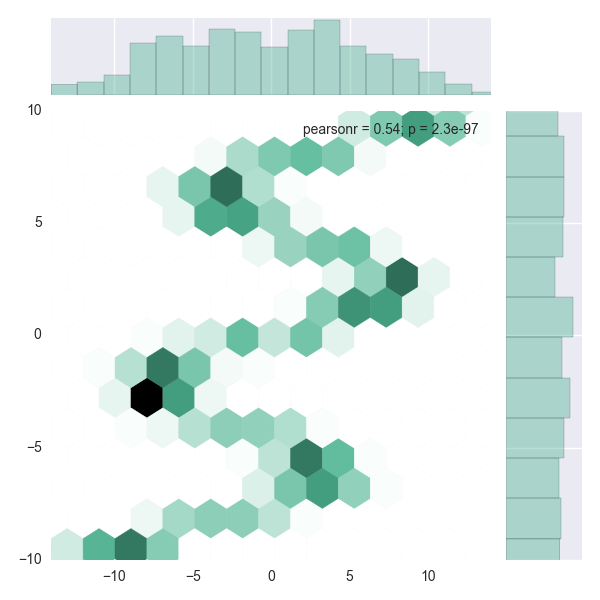
\includegraphics[width=700px]{/images/mdn-fig3.png}

\subsubsection{Acknowledgments}

We are grateful to Christopher Bonnett for writing the initial version
of this tutorial. More generally, we thank Chris for pushing forward
momentum to have Edward tutorials be accessible and easy-to-learn.

\subsubsection{References}\label{references}
